% FILENAME: doc.tex
% AUTHOR: Zachary Krepelka
% DATE: Wednesday, January 17th, 2024
% ABOUT: documentation for my server-side programming class
% ORIGIN: https://github.com/zachary-krepelka/server-side_programming.git
% COMPILATION: texfot pdflatex --halt-on-error -shell-escape doc.tex

%%%%%%%%%%%%%%%%%%%%%%%%%%%%%%%%%%%%%%%%%%%%%%%%%%%%%%%%%%%%%%%%%%%%%%%%%%%%%%%%

%  ___                    _    _
% | _ \_ _ ___ __ _ _ __ | |__| |___
% |  _/ '_/ -_) _` | '  \| '_ \ / -_)
% |_| |_| \___\__,_|_|_|_|_.__/_\___|

\documentclass{article}

\title{Server-side Programming}
\author{Zachary Krepelka}
\date{Wednesday, January 17th, 2024}

\usepackage{algpseudocode}
\usepackage{csquotes}
\usepackage{enumitem}
\usepackage{graphicx} \graphicspath{ {images/} }
\usepackage{minted} \setminted{bgcolor=lightgray!20!white}
\usepackage{url}

%%%%%%%%%%%%%%%%%%%%%%%%%%%%%%%%%%%%%%%%%%%%%%%%%%%%%%%%%%%%%%%%%%%%%%%%%%%%%%%%

%  _____ _ _   _       ___
% |_   _(_) |_| |___  | _ \__ _ __ _ ___
%   | | | |  _| / -_) |  _/ _` / _` / -_)
%   |_| |_|\__|_\___| |_| \__,_\__, \___|
%                              |___/

\begin{document}
\maketitle
\tableofcontents
\newpage
\listoflistings
\listoffigures
\newpage

%%%%%%%%%%%%%%%%%%%%%%%%%%%%%%%%%%%%%%%%%%%%%%%%%%%%%%%%%%%%%%%%%%%%%%%%%%%%%%%%

%  ___     _               _         _   _
% |_ _|_ _| |_ _ _ ___  __| |_  _ __| |_(_)___ _ _
%  | || ' \  _| '_/ _ \/ _` | || / _|  _| / _ \ ' \
% |___|_||_\__|_| \___/\__,_|\_,_\__|\__|_\___/_||_|

% I want the section numbering to coincide with the number of the assignment.
% Because of this, the introduction is left unnumbered. Subsections under the
% introduction are also unnumbered.

\section*{Introduction}
\addcontentsline{toc}{section}{Introduction}

This semester I am taking a classed called `Server-side Programming' at Saint
Francis University. The purpose of this document is to journal my assignments as
per the requirements of the class:

\begin{quote}

	Provide technical documentation for each of the assignments thus far
	detailing the installation/configuration process with text descriptions
	and screenshots.  The document should be able to be taken by a
	semi-technical individual to complete each assignment without
	assistance. ---Dr.\ Slonka

\end{quote}

%-------------------------------------------------------------------------------

\subsection*{Organization}
\addcontentsline{toc}{subsection}{Organization}

Each assignment is documented within its own section of this document.  To
provide context, the assignment is reproduced verbatim.  Thereafter, the
remaining content within each section is subdivided into subsections.  They may
include, but are not limited to, the following.

\begin{itemize}

	\item

		\emph{Background.} This subsection details preliminary research
		and elaborates on keywords within the assignment. \emph{Context}
		is provided here.

	\item

		\emph{Where I Stand.} Here I remark if I have had prior
		experience with any aspect of the assignment. This information
		can aid the reader; it helps to know where the author stands.

	\item

		\emph{Steps.} These subsections detail the steps required to
		complete the assignment. They are numbered as necessary.

	\item

		\emph{Resources.} Here I list the resources I accessed to
		research the assignment. This subsection entails a bulleted list
		of URLs.

\end{itemize}

%-------------------------------------------------------------------------------

\subsection*{Assumptions}
\addcontentsline{toc}{subsection}{Assumptions}

We make the following assumptions about the reader.

\begin{itemize}

	\item

		The reader is working on a Linux machine.  We will be using a
		Ubuntu virtual machine with Oracle VM VirtualBox as our
		hypervisor. It is assumed that the operating system is already
		installed and set up. Instructions can be found online.

	\item

		The reader has rudimentary competency at the command line. The
		reader knows how to open a terminal and issue basic commands
		like \verb|ls| or \verb|cd|.

\end{itemize}

%-------------------------------------------------------------------------------

\subsection*{Typographical Conventions}
\addcontentsline{toc}{subsection}{Typographical Conventions}

Screenshots are reserved for graphical user interfaces.  I don't see any good
reason to provide screenshots of terminal commands since they are entirely text.
Instead, I will prefer to provide shell commands in a textual format. They will
appear as follows.  To clearly distinguish input from output, the result of the
command is indented whereas the command itself is left justified and prefixed
with a dollar sign.
%
\begin{minted}{text}
$ grep author doc.tex

	\author{Zachary Krepelka}
\end{minted}
%stopzone https://tex.stackexchange.com/a/618003
%
In other circumstances, however, the output is omitted entirely, like this:
\mint{text}{$ sed 's/\(Zachary\) \(Krepelka\)/\1 Paul \2/' doc.tex} %stopzone
%
It is also possible for shell commands to appear inline, like this:
\mintinline{bash}{less doc.tex}.  Listing \ref{listing:totatives} is included to
provide an example of how code will appear throughout this document.  Take
notice the numbers on the side of Listing \ref{listing:totatives}. These can be
used to identify and discuss specific lines of code. Longer programs will be
built up incrementally with commentary dispersed throughout, and a final listing
will be provided thereafter.

\begin{listing}[h]
\begin{minted}[frame=lines, linenos]{ruby}
#!/usr/bin/env ruby

# FILENAME: totatives.rb
# AUTHOR: Zachary Krepelka
# DATE: Wednesday, November 29th, 2023

class Integer
    def totatives
        fail unless positive?
        1.upto(self).select do |i|
            gcd(i) == 1
        end
    end
end
\end{minted}
\caption{a Ruby program to compute the set of totatives of a number.}
\label{listing:totatives}
\end{listing}

%-------------------------------------------------------------------------------

% \subsection*{Integrity}
% \addcontentsline{toc}{subsection}{Integrity}

% One final remark: to ensure the integrity of this documentation, I will be
% re-working through each assignment on a fresh instance of a Ubuntu VM.

%%%%%%%%%%%%%%%%%%%%%%%%%%%%%%%%%%%%%%%%%%%%%%%%%%%%%%%%%%%%%%%%%%%%%%%%%%%%%%%%

%    _          _                         _       _ _    __
%   /_\   _____(_)__ _ _ _  _ __  ___ _ _| |_   _| | |_ /  \
%  / _ \ (_-<_-< / _` | ' \| '  \/ -_) ' \  _| |_  .  _| () |
% /_/ \_\/__/__/_\__, |_||_|_|_|_\___|_||_\__| |_     _|\__/
%                |___/                           |_|_|

\newpage

\setcounter{section}{-1}

% Start the section numbering at zero.
% This first assignment doesn't really count.
% It was a preliminary matter that did not entail any programming.
% All subsequent assignemnts will be numbered from one onwards.

\section{Git}

Our first assignment asked us to set up a GitHub repo for this class.

\begin{enumerate}

	\item Create a GitHub account (if you don't already have one).

	\item Create a directory on your Linux VM for your CPSC222 assignments.

	\item Create a repo in that folder.

	\item Create a README file in that folder that contains your name.

	\item Push your changes to the repo.

	\item

		Submit your repo URL so that the professor can clone your repo
		and see your files.

\end{enumerate}

%-------------------------------------------------------------------------------

\subsection{Background}

Git is a version control system that tracks changes in computer files.  It was
originally authored by Linus Torvalds, the creator of the Linux kernel. GitHub,
which is built on top of Git, is an online platform for software developers to
store, manage, share, and collaborate on code.

%-------------------------------------------------------------------------------

\subsection{Where I Stand}

I already had a GitHub account prior to coming into this class, and I was
already familiar with the basic Git terminal commands. Because I don't remember
the specific steps involved in signing up, I will be creating a burner account
on GitHub with a temporary email for the purpose of writing this documentation.

%-------------------------------------------------------------------------------

\subsection{Steps}

We work through the steps as specified.

\subsubsection{Account Creation}

Step \#1 of this assignment asks us to create an account with GitHub.

\begin{enumerate}

	\item

		Begin by pointing your web browser to
		\url{https://github.com/signup}.  You will be met with a page as
		shown in Figure \ref{fig:adventure} that asks you to enter your
		new account credentials, viz., email, password, username, and
		email preferences. You will also be asked to verify that you are
		not a robot by preforming a small puzzle.  To proceed, click on
		the text fields indicated by the pink arrows. After you have
		entered your email and new password, click `Create Account'. Be
		sure to create a strong password. Write down your account
		credentials for save keeping.

	\item

		Next you will be brought to a page as shown in Figure
		\ref{fig:almost-done} that asks you to enter a verification code
		sent to your email. Access your email, retrieve the code, type
		it in, and continue.

	\item

		The next pages asks you to personalize your account by supplying
		information about your demographics, e.g., student, teacher,
		N/A. For our purposes, we will be skipping the personalization
		by clicking the `Skip personalization' button. However, if you
		are a student, you should fill this section out because GitHub
		will provide free educational access to certain tools and
		technologies. See Figure \ref{fig:skip-personalization}.

	\item

		You are now at your GitHub dashboard, as shown in Figure
		\ref{fig:homepage}. From here, you'll want to click on the big,
		bright green button in the top left-hand corner of the screen
		that says `Create repository.' You will be taken to a page as
		shown in Figure \ref{fig:new-repo}. You'll wnat to give your
		repository a name and description. Then choose whether you want
		a private or public repository. We will choose to make a public
		repository. You can ignore everything else. We will add a README
		file later. When everything has been filled out, click `Create
		repository.'

	\item

		After creating your repository, you will be brought to a quick
		setup page as shown in Figure \ref{fig:quick-setup}. There will
		be a blue box containing your new GitHub repositorie's URl. Copy
		this to your clipboard and save it for later.  You will see that
		there are instructions for creating a repositiory or pushing an
		existing repository from the command line. We will walk though
		this in the next subsection.  At this point, you can savely
		close the window.

\end{enumerate}

\subsubsection{Directory Creation}

Step \#2 of this assignment asks us to create a directory to store our
assignments for this class. Begin by opening a terminal on your Linux machine.
This can be done by pressing \verb|CTRL-ALT-T| on your keyboard, but it will
also suffice to find the terminal by searching through the available software.
This can be done by clicking the grid icon in the bottom left-hand corner of the
screen of the Ubuntu desktop as shown in Figure \ref{fig:ubuntu-desktop}.  Once
the terminal command is open, issue the following command.
%
\mint{text}{$ cd Documents} %stopzone
%
This will change our current working directory to the documents folder.  This is
where we will be storing our code, but you can choose another location if you
wish. The command should return silently, indicating success. Next you will want
to make a new directory as instructed in the assignment. Do this by issuing the
following command.
%
\mint{text}{$ mkdir ssp; cd ssp} %stopzone
%
The \verb|mkdir| command will create a new subdirectory in the user's current
working directory (or elsewhere if specified). Its first positional argument is
the name of the new directory, which we have chosen to be `ssp' as an acronym
for `server-side programming.' The semicolon is a \emph{command separator}.

\subsubsection{Local Repo Creation}

Step \#3 of this assignment asks us to create a local Git repository in the
directory we created in step \#2. Recall that Git and GitHub are distinct
entities as previously discussed. Our new Git repo will be local to our machine.
First ensure that Git is installed on this system by typing
\mintinline{bash}{which git}. This command will point to the Git's executable
binary if it exists. If the command returns nothing, you will need to install
Git using your installation method of choice. Since we are using Ubuntu, we will
use its default package manager by typing the following command.
%
\mint{bash}{$ sudo apt install git -y} %stopzone
%
The \verb|-y| flag instructs the \verb|apt| package manager to install the
software without user intervention. Without it, the user would have to type `y'
for ``yes, I want to install this software.'' After installation, the terminal
will be cluttered with installation information, so you can type
\mintinline{bash}{clear} to clear your terminal.
%
You will also need to set up git. Tell Git your name like this.
%
\mint{bash}{$ git config --global user.name "Joe Smith"} %stopzone
%
Tell Git your email like this.
%
\begin{minted}{bash}
$ git config --global user.email \
"162062323+throw-away-account-123@users.noreply.github.com"
\end{minted}
%stopzone
%
Here the backslash is used for line continuation.  You likely won't want to use
your personal email when uploading changes to GitHub.  For this reason, GitHub
provides a special noreply email to hide your real email. To figure out yours,
point your web browser to \url{github.com/settings/emails}, first ensuring that
you are signed in. There you will find your new noreply email under the `Keep my
email addresses private' checkbox as shown in Figure \ref{fig:noreply-email}.
You'll want to ensure that that check mark box is selected.  To ensure the
process worked, you can type \mintinline{bash}{cat ~/.gitconfig} to preview your
Git dotfile. It should look similar to mine.
%
\begin{minted}{text}
[user]
	name = Joe Smith
	email = 162062323+throw-away-account-123@users.norepl...
\end{minted}

Now we are ready to create the local Git repository.  Once again confirm that
you are in the directory you wish to initialize a repo in by typing
\mintinline{bash}{pwd}. Then type \mintinline{bash}{git init} to create a Git
repository in the current working directory. Typing \mintinline{bash}{ls -a}
will confirm that a hidden Git directory is present.  Git will use this
directory to keep track of changes in your project.

\subsubsection{Creating a README}

Step \#4 of this assignment asks us to create a README file.  Create a README
file by typing \mintinline{bash}{touch REAME.md}. Then edit the file using your
text editor of choice. The nano text editor is a good choice for beginners, and
you can use it by typing \mintinline{bash}{nano README.md}\footnote{The touch
command is not necessary. If supplied with a name on startup, the text editor
will automatically create the file when it is saved for the first time.}. Add
the following lines.

\begin{minted}{markdown}
# Server-side Programming
My name is Joe Smith.
\end{minted}

The README file uses a markup language called Markdown to specify the appearance
and content of the document. The README file will be rendered in the web browser
when others visit your GitHub page, but Markdown is also designed to be readable
from the terminal as plaintext. We will not go into detail here on how to write
Markdown. The reader will find plenty of tutorials on the internet.

I will not explain the Git life cycle here in detail. For now, it will suffice
to remark that Git works by \emph{staging} changes in files. Thereafter, the
changes can be finalized by \emph{committing} them. By doing this, the user is
able to track the change history of a project. The commits serve as way point
markers in a project's history. Git does a lot more than this, but this is all
we need to know for now.

To stage your new file for a commit, type \mintinline{bash}{git add README.md}.
Follow this by \mintinline{bash}{git commit -m 'first commit'} to commit your
changes. The \verb|-m| flag specifies a message describing the commit. Be
mindful when authoring commit messages. A Google search for `commit message
guidelines' is recommended.

Git's default branch (I will not explain branches here) used to be called
`master.' For political correctness, GitHub encourages you to change your
default branch name to `main.' This can be done by typing \mintinline{bash}{git
branch -M main}. You can call the main branch whatever you want.

You have successfully created a local Git repository.

\subsubsection{Uploading to the Cloud}

Now we complete Step \#5 of the assignment.  To share your code online with
other people, you can link your local Git repo with an online platform like
GitHub. Issue this command.
%
\mint{bash}{git remote add origin [YOUR GITHUB REPO URL HERE FROM STEP 1]}
%
Mine looks like this.
%
\mint{text}{https://github.com/throw-away-account-123/throw-away-repo.git}
%
This command only establishes a relationship. To actually store your code in the
remote repository, you'll want to push the changes to the cloud, like this.
%
\mint{bash}{git push -u origin main}
%
But we're not done yet.  You have to supply your username and password for the
remote repository. GitHub does not let you use your account password, so you
have to create what is called an \emph{access token}.  Point your web browser to
\url{https://github.com/settings/tokens/new} and enter your account password if
required. You will be brought to a page as shown in Figure \ref{fig:token}.
Enter a description for your token under the note text field. Then check mark
the appropriate boxes. It is often easier to just check mark them all if you are
unsure. Once you have done this, click the bright green `Generate token' button
at the bottom of the page.  The token will then be available for you to copy as
shown in Figure \ref{fig:access-token-copy-and-paste}.  Write it down for save
keeping. You will have to periodically regenerate your access token.  Use this
as your password for the \mintinline{bash}{git push} command.

%-------------------------------------------------------------------------------

\subsection{Resources}

GitHub's quick start guide is a good place to start.
%
\begin{center}
	\url{https://docs.github.com/en/get-started/start-your-journey}
\end{center}
%
It will walk you through the basics of Git and GitHub. You will be asked to
create a `hello-world' repository.

%-------------------------------------------------------------------------------

% Images

\begin{figure}[p]
	\centering
	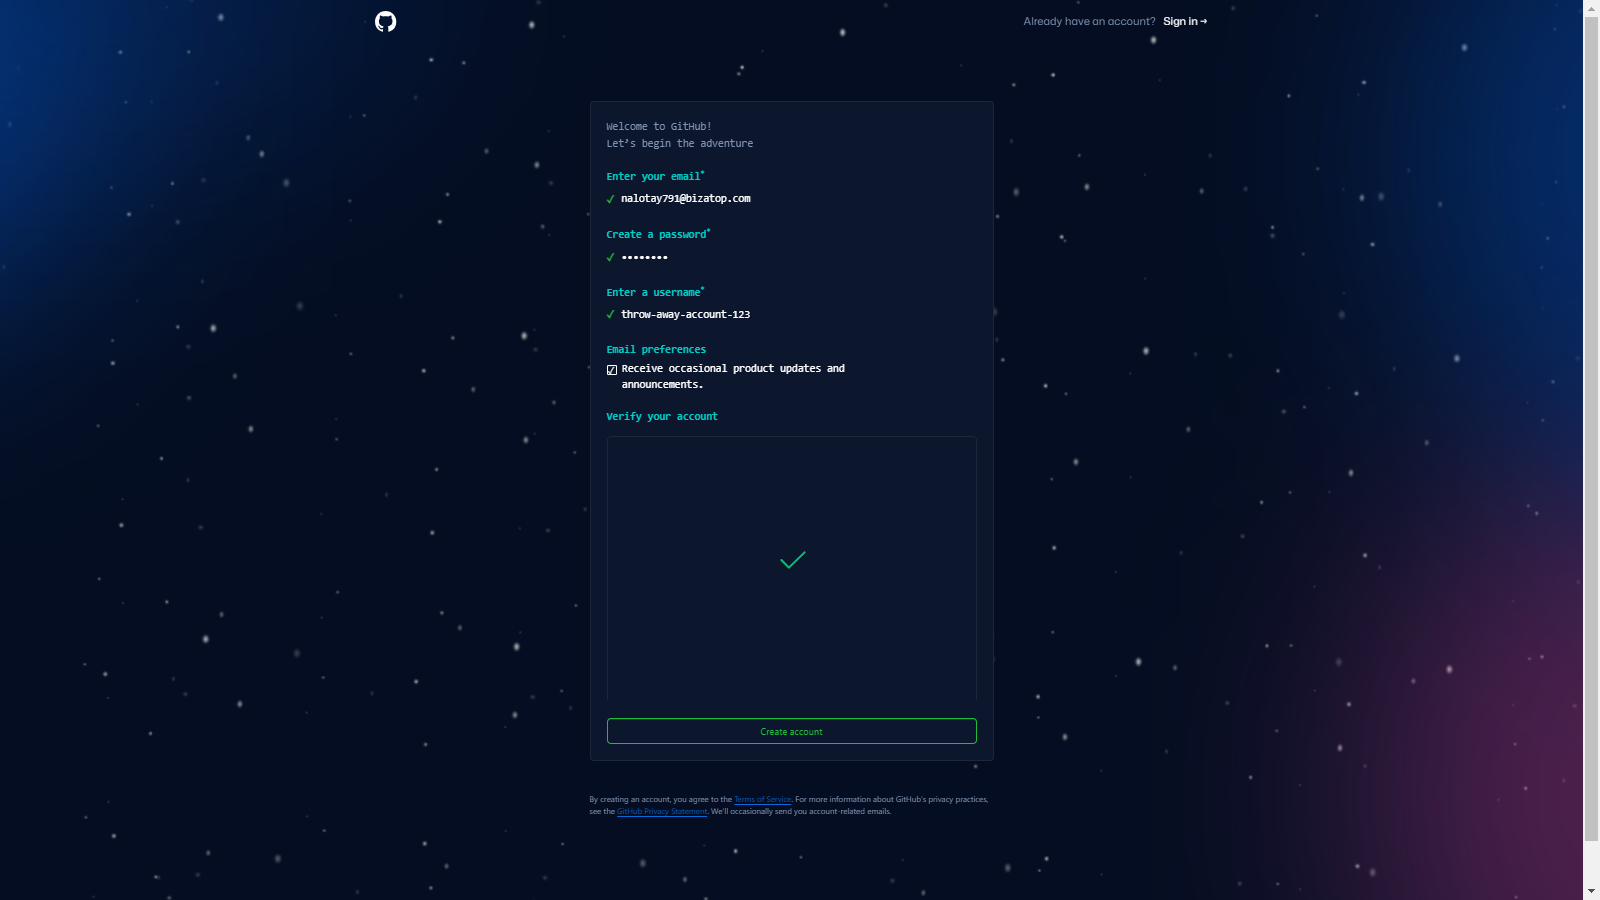
\includegraphics[width=\textwidth]{adventure.png}
	\caption{GitHub's Signup Page.}
	\label{fig:adventure}
\end{figure}

\begin{figure}[p]
	\centering
	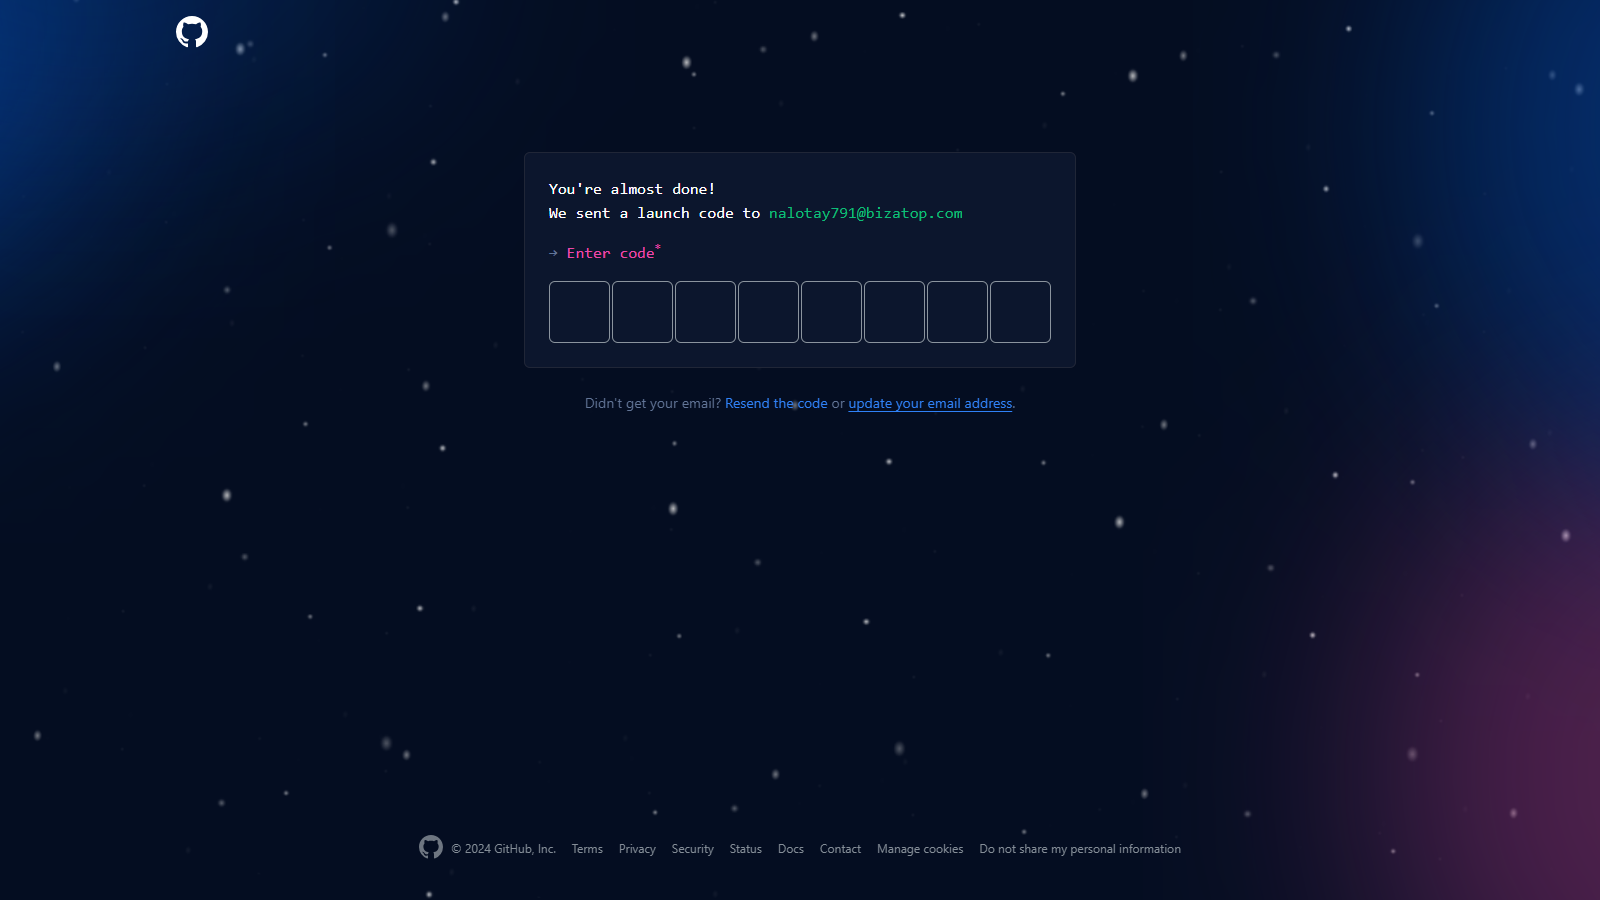
\includegraphics[width=\textwidth]{almost-done.png}
	\caption{GitHub's Email Verification Page.}
	\label{fig:almost-done}
\end{figure}

\begin{figure}[p]
	\centering
	
\includegraphics[width=\textwidth]{skip-personalization.png}
	\caption{GitHub's Personalization Page.}
	\label{fig:skip-personalization}
\end{figure}

\begin{figure}[p]
	\centering
	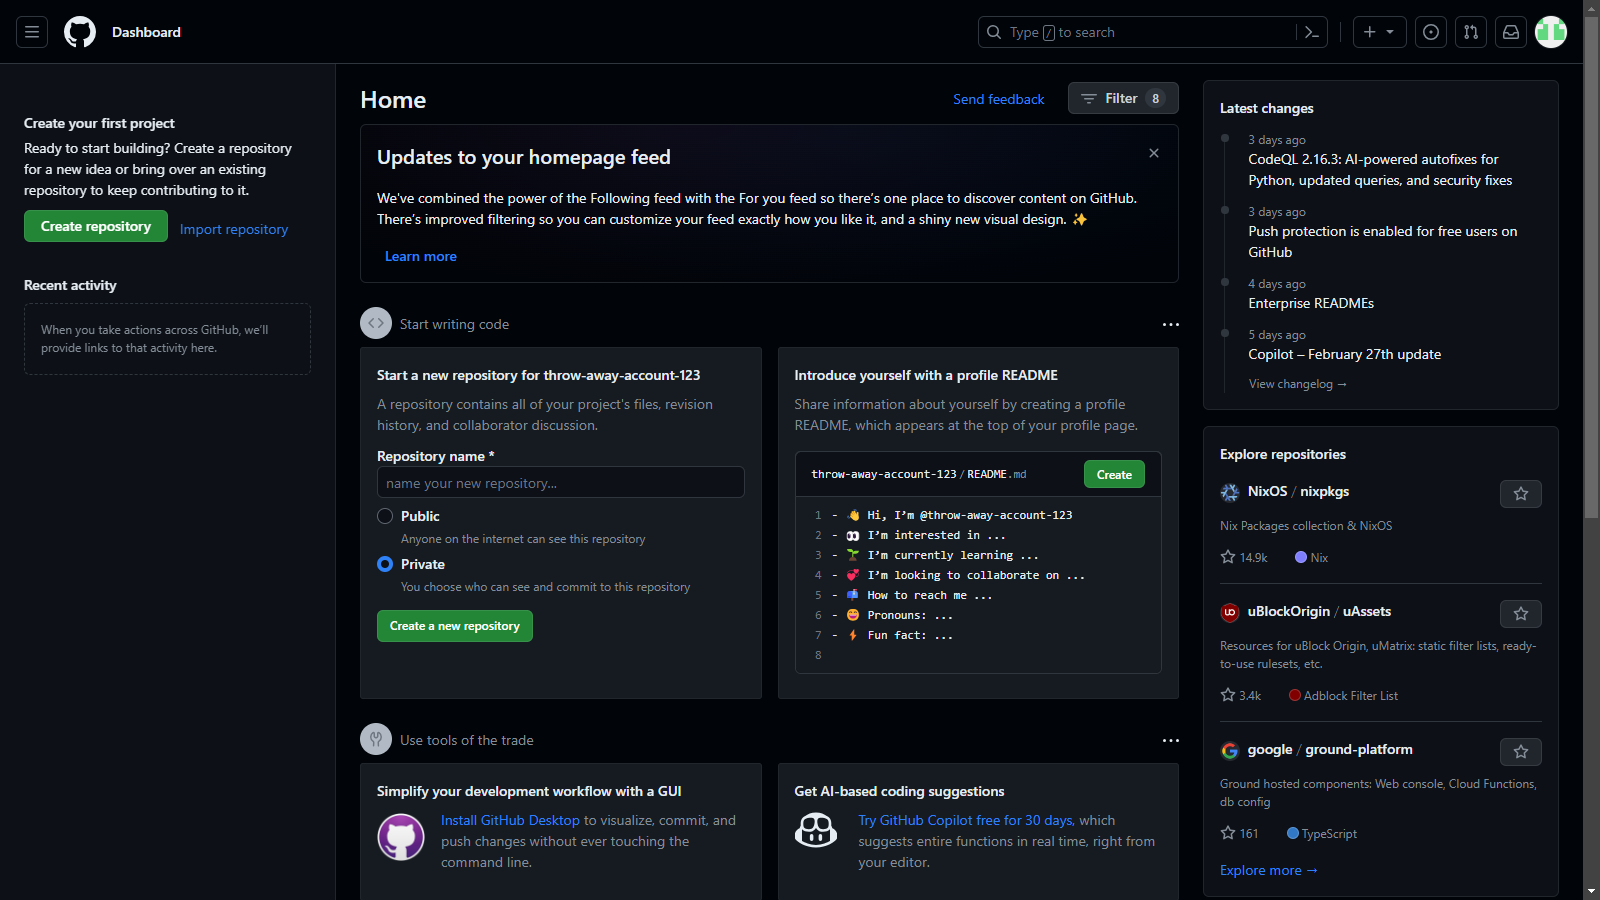
\includegraphics[width=\textwidth]{homepage.png}
	\caption{The GitHub Dashboard.}
	\label{fig:homepage}
\end{figure}

\begin{figure}[p]
	\centering
	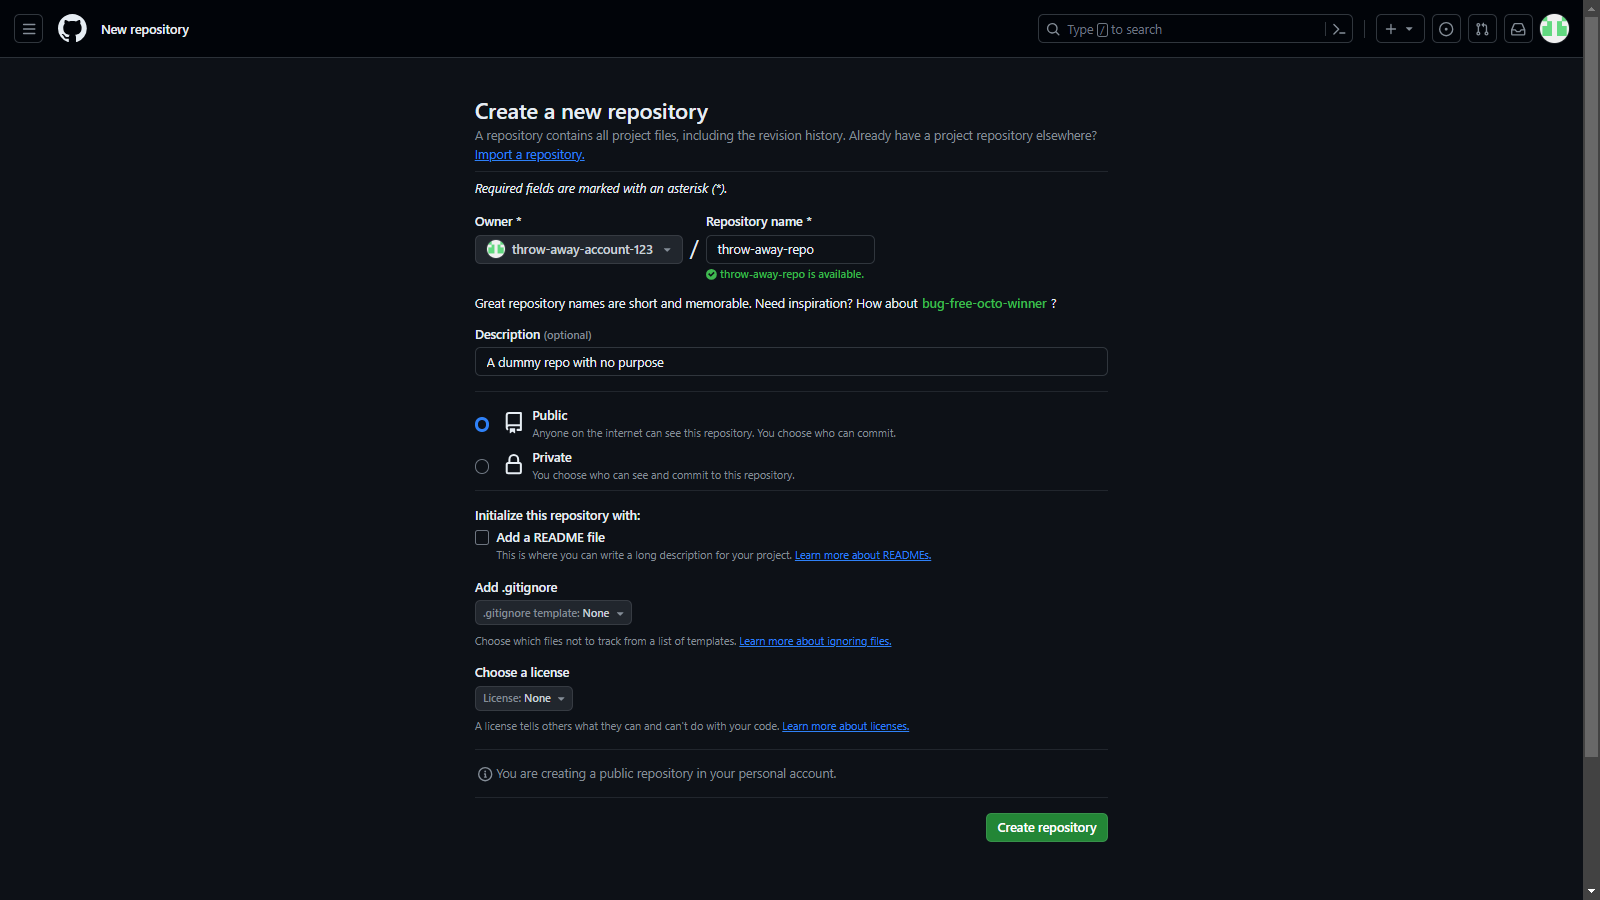
\includegraphics[width=\textwidth]{new-repo.png}
	\caption{GitHub's Repository Creation Page.}
	\label{fig:new-repo}
\end{figure}

\begin{figure}[p]
	\centering
	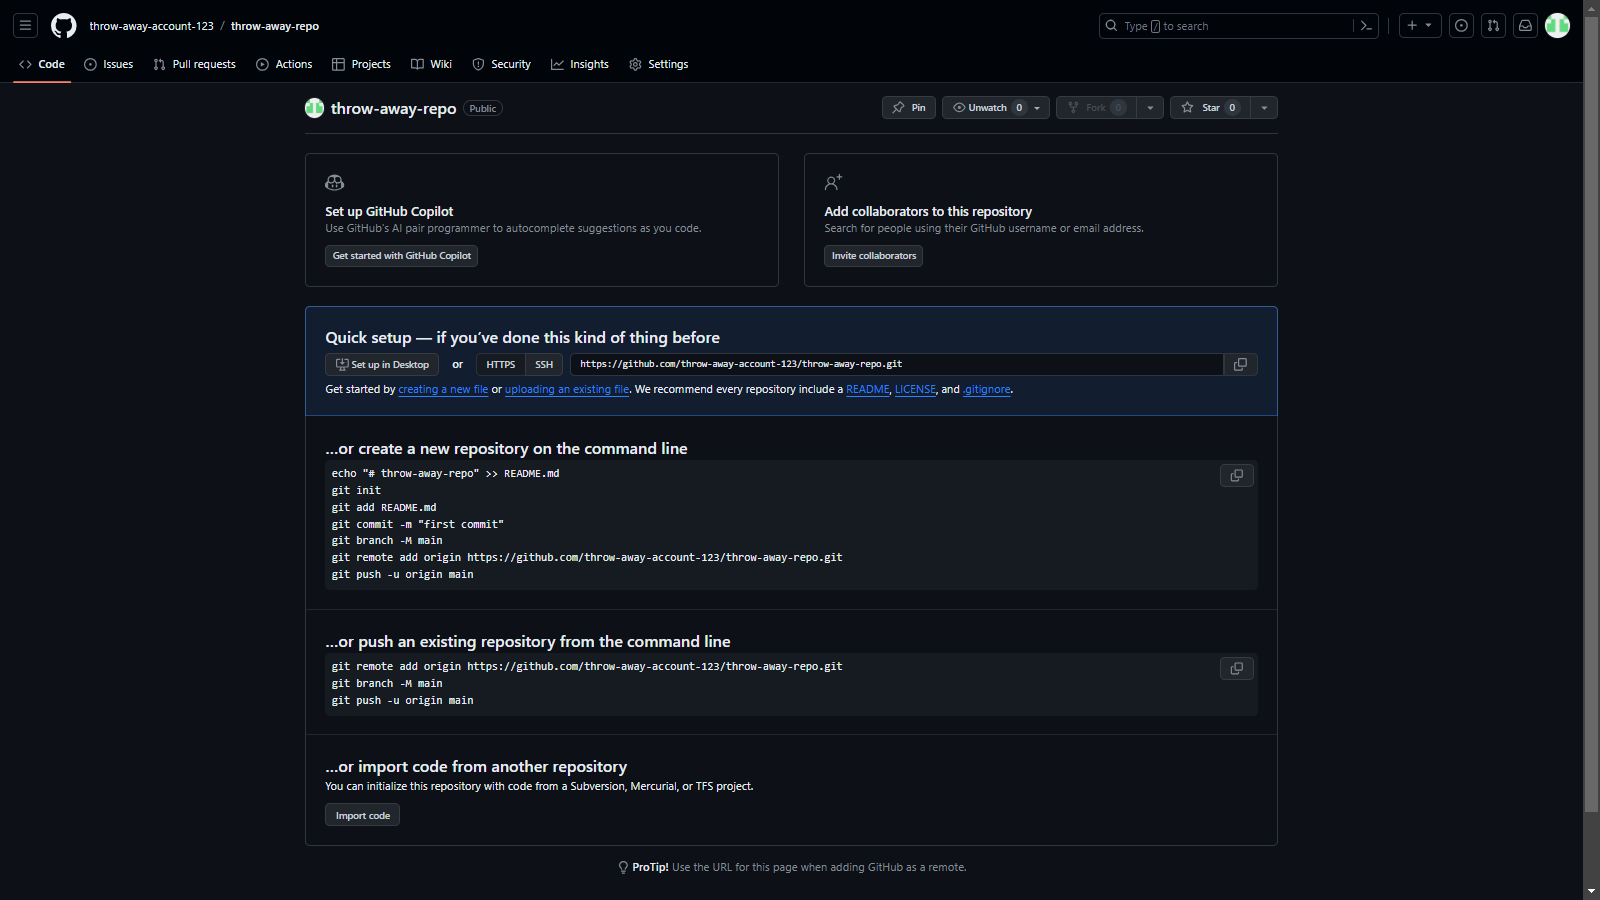
\includegraphics[width=\textwidth]{quick-setup.png}
	\caption{GitHub's Quick Setup Page for a New Repository.}
	\label{fig:quick-setup}
\end{figure}

\begin{figure}[p]
	\centering
	
\includegraphics[width=\textwidth]{ubuntu-desktop.png}
	\caption{The Ubuntu Desktop.}
	\label{fig:ubuntu-desktop}
\end{figure}

\begin{figure}[p]
	\centering
	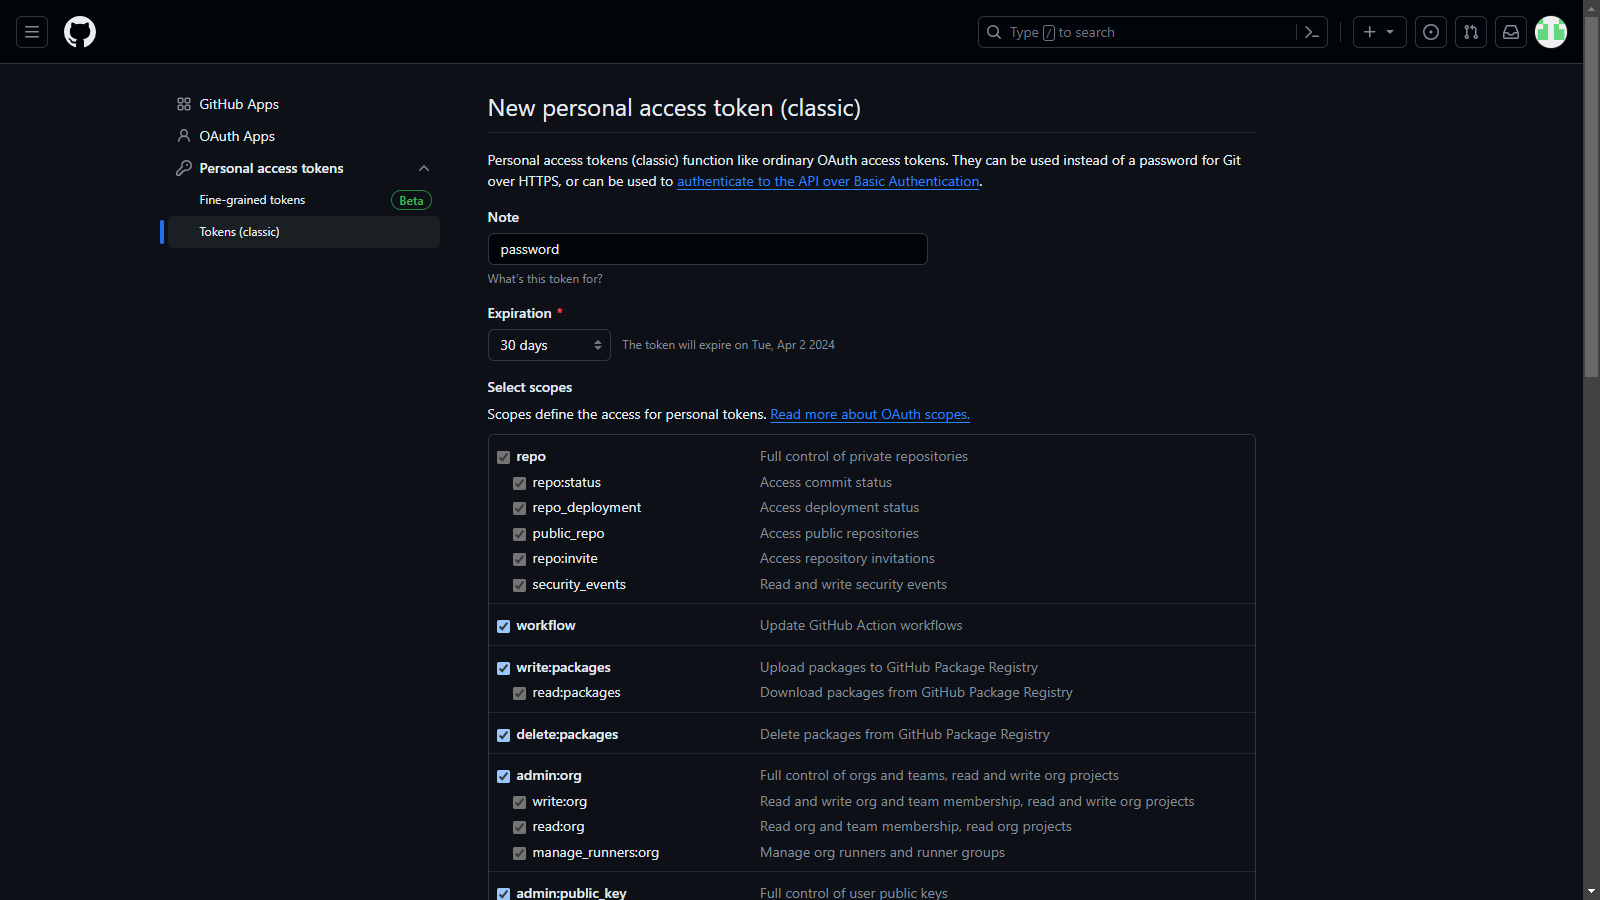
\includegraphics[width=\textwidth]{token.png}
	\caption{GitHub's Personal Access Token Creation Page.}
	\label{fig:token}
\end{figure}

\begin{figure}[p]
	\centering
	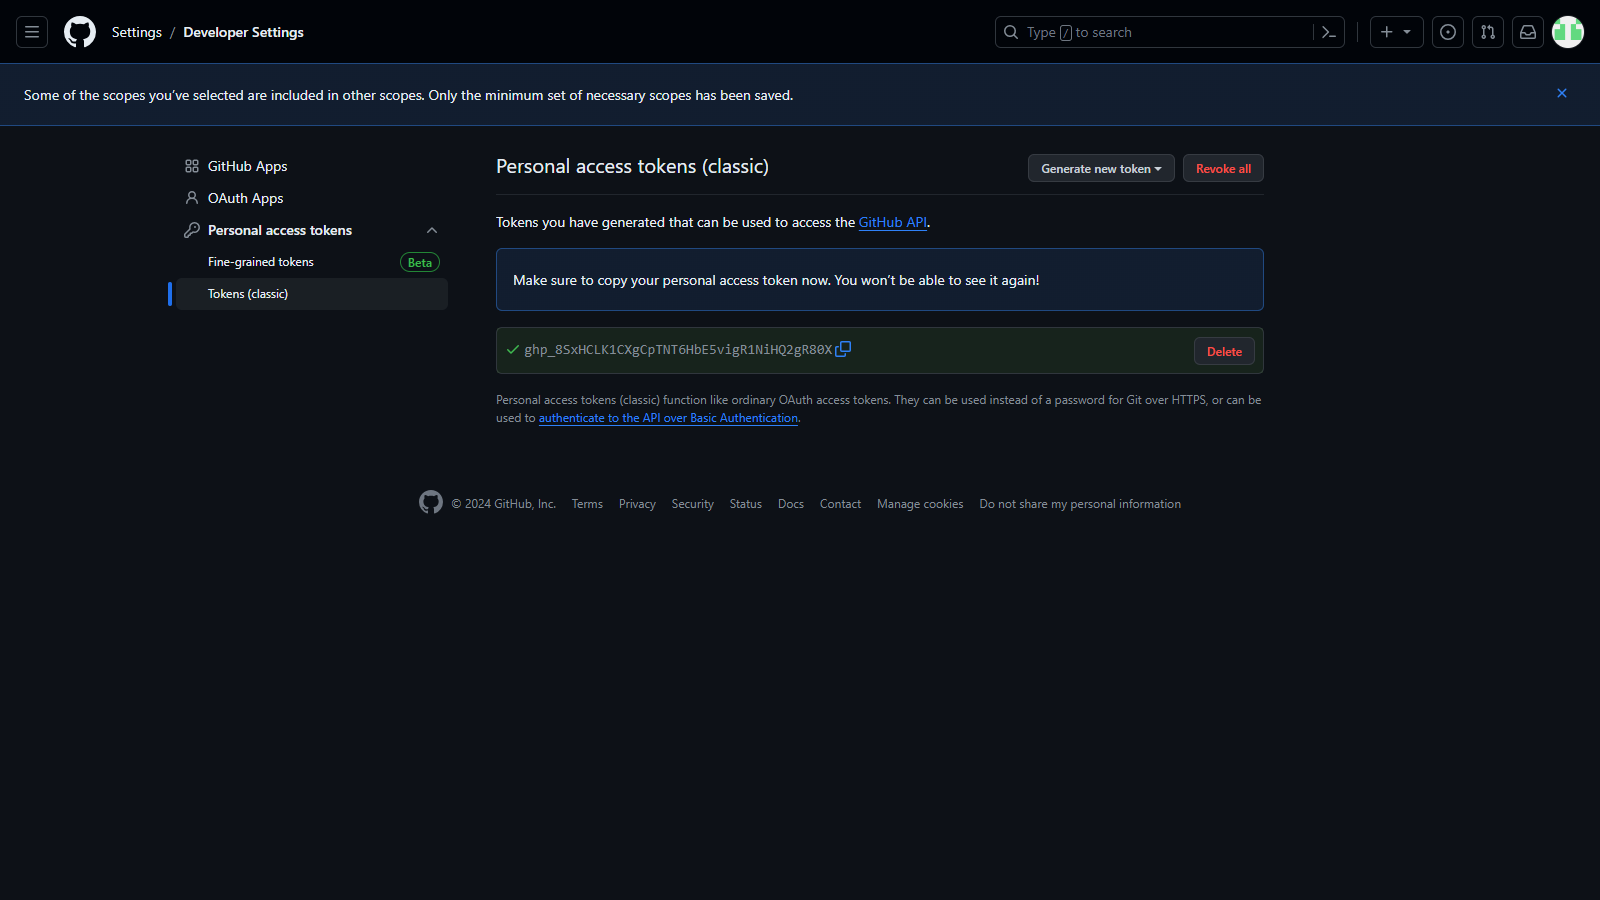
\includegraphics[width=\textwidth]{access-token-copy-and-paste.png}
	\caption{An Example of a Personal Access Token.}
	\label{fig:access-token-copy-and-paste}
\end{figure}

\begin{figure}[p]
	\centering
	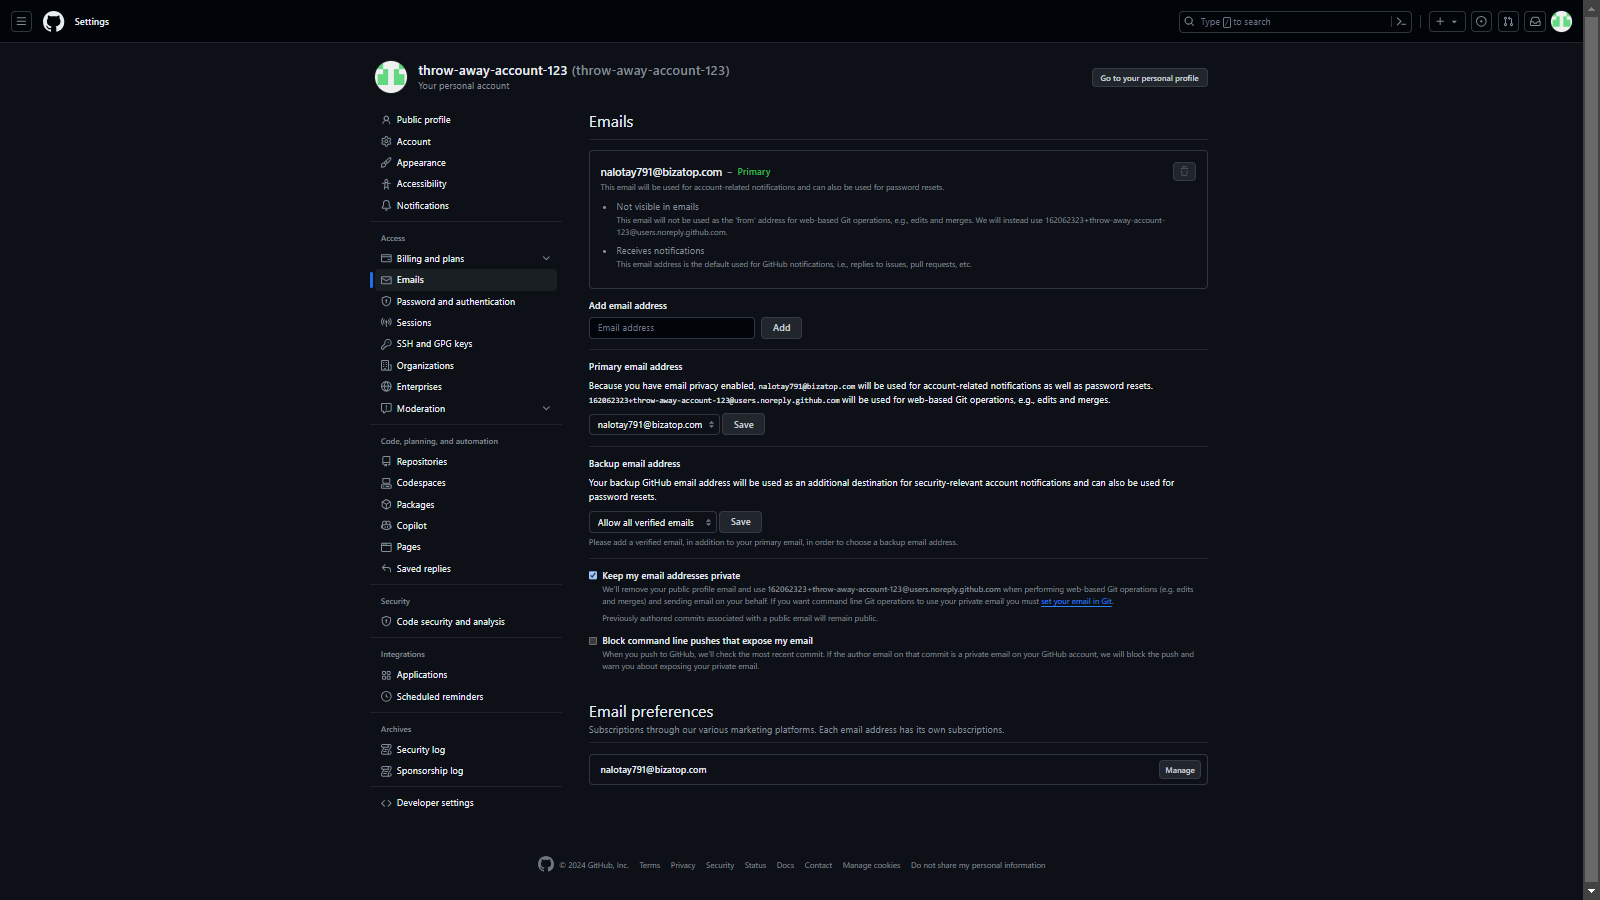
\includegraphics[width=\textwidth]{noreply-email.png}
	\caption{GitHub's Email Settings Page.}
	\label{fig:noreply-email}
\end{figure}

\clearpage

%%%%%%%%%%%%%%%%%%%%%%%%%%%%%%%%%%%%%%%%%%%%%%%%%%%%%%%%%%%%%%%%%%%%%%%%%%%%%%%

%    _          _                         _       _ _   _
%   /_\   _____(_)__ _ _ _  _ __  ___ _ _| |_   _| | |_/ |
%  / _ \ (_-<_-< / _` | ' \| '  \/ -_) ' \  _| |_  .  _| |
% /_/ \_\/__/__/_\__, |_||_|_|_|_\___|_||_\__| |_     _|_|
%                |___/                           |_|_|

\section{SNMP sudo usage}

Our first non-trivial assignment follows. % Which is why it's number 1.

\begin{enumerate}

	\item

		Write a Perl script that produces the number of successful sudo
		sessions on your host. The output shall only be a number without
		a trailing newline.

	\item Make this script's results available via SNMP.

\end{enumerate}
%
Add your script and snmp config file to your git repo and submit your repo URL
and the command to prove that you can read the result via SNMP.

%-------------------------------------------------------------------------------

\subsection{Background}

Three words stand out: SNMP, Perl, and sudo. Let's discuss each.

\subsubsection{SNMP}

It stands for simple network management protocol.  In general, a communication
protocol is a set of rules used to coordinate computers so they know how to
interact with each other. An important point is that a protocol is not a piece
of software.  Rather, a protocol is a specification published in a formal
document, put together by a committee of people.  Be that as it may, a
communication protocol needs to be implemented in software to be useful.  For
example, one should distinguish between  the Secure Shell protocol, which is a
set of rules, and the software implementing that protocol, like
\verb|openssh-client| and \verb|openssh-server| on Linux.

In this assignment, we will be using the simple network management protocol,
which is a networking protocol for monitoring and managing devices on a
%
network\footnote{\url{https://askubuntu.com/a/252994}}.
%
In this explanation, I will focus on the monitoring aspect.  A standard use case
is to access information about a remote computer, e.g., the speed of a fan, the
temperature of a CPU, the host name of the device, etc.  The SNMP protocol
structures this information in a tree database called a \emph{management
information base} (MIB). It can be likened to a file tree. Because the
information that SNMP monitors and manages often pertains to proprietary
hardware, SNMP can be expanded with third-party MIB files. For copyright
reasons, these are usually not included by default on Linux systems having SNMP
software pre-installed. The individual nodes in a MIB tree are identified and
accessed with Object Identifiers, or OIDs for short.

\subsubsection{Perl}

The SNMP protocol can be extended to expose the results of a script. In this
assignment, we will be writing a Perl script to use in conjunction with SNMP.
Perl is a scripting language with close ties to the Unix family of tools, e.g.,
sed, AWK, sh, and C. It's well known for its text processing capabilities and
powerful regular expression engine. It was created in 1987 by Larry Wall.

\subsubsection{Sudo Session}

Linux permissions work in part by granting the user temporary access to elevated
privileges only when they are
%
necessary\footnote{\url{%
https://en.wikipedia.org/wiki/Principle_of_least_privilege}}.
%
This is done by prefixing a command with the command \verb|sudo|, for `super
user do.'  The duration of time that the user has elevated privileges is called
the sudo session.  That way, commands that require sudo privileges can be issued
in succession without adding sudo to every one\textemdash imagine reentering
your password every time! A quick Google search tells us that a standard sudo
session lasts for 5 minutes.

%-------------------------------------------------------------------------------

\subsection{Where I Stand}

I have some limited prior experience with Perl, but I didn't know anything about
SNMP before this assignment.

%-------------------------------------------------------------------------------

\subsection{Steps}

We address the two components of the assignment separately.

\subsubsection{Writing the Perl Script}

Before we even touch the keyboard, we should plan out our program in advance.
How will we find the number of sudo sessions?  A few Google searches will tell
us to look in
%
\verb|/var/log/auth.log|\footnote{https://unix.stackexchange.com/q/167935}.
%
This is a log file containing information about \emph{authorization} attempts on
the system. A careful study of this file will reveal that sudo sessions are
recorded on lines containing the strings \verb|sudo:session| and \verb|opened|.
Hence, our script must count the occurrences of lines in
\verb|/var/log/auth.log| containing both \verb|sudo:session| and \verb|opened|,
although there are surely other ways to do it.  We express our plan as
pseudocode in Listing \ref{listing:sudo-session-pseudocode}.

\begin{listing}[h]
\hrule \vspace{1em}
\begin{algorithmic}[1]
\Require authorization log file present and accessible on system
\Ensure number as a string with no trailing newline
\State{$count \gets 0$}
\For{\textit{line} \textbf{in} \textit{authorization log file}}
	\If{%
		\textit{line} contains `sudo:session' \textbf{and}
		\textit{line} contains `opened'
	}
		\State{$count \gets count + 1$}
	\EndIf
\EndFor
\State \textbf{output} $count$
\end{algorithmic}
\vspace{1em} \hrule
\caption{pseudocode for sudo session script}
\label{listing:sudo-session-pseudocode}
\end{listing}

\paragraph{Shell Script}

As a preliminary exercise, it is not hard to cook up a standard shell script to
implement our plan.  In fact, it can be done quite succinctly as shown in
Listing \ref{listing:sudo-session-shell-script}. Let's go through it together.

\begin{itemize}[leftmargin=*]

	\item

		\textbf{line 1} The first line contains an interpreter
		directive called a \emph{shebang}. It tells the system which
		binary to use to execute the program, in this case
		\verb|/bin/sh|.

	\item

		\textbf{line 7} Skipping over the comments, we first search
		for the string `sudo:session' in our \verb|auth.log| file using
		grep, a standard Unix command-line program whose name is an
		acronym for `global regular expression print.'

	\item

		\textbf{line 8} After searching for the `sudo:session' string,
		we search for the `opened' string in lines already containing
		the `sudo:session' string.  This is accomplished by
		\emph{piping} the first search command into the second.  Piping
		is the process of redirecting the output of one command as input
		into another command; it is signified by the vertical bar.
		Hence, the second grep command searches within the output of the
		first grep command. In effect, this captures lines in the
		original file containing both strings.

	\item

		\textbf{line 9} The resulting output, which only contains the
		lines having other search strings, is then piped into the word
		count command \verb|wc| with the flag \verb|-l| to determine the
		number of lines.

	\item

		\textbf{line 10} Finally, that number result is piped into the
		translate command \verb|tr| with the \verb|-d| command to
		\emph{delete} the trailing newline.

\end{itemize}

Our implementation in Listing \ref{listing:sudo-session-shell-script} looks
quite different from our pseudo code in Listing
\ref{listing:sudo-session-pseudocode}, but they are not so different; the
for-loop is buried inside the grep command, and the logical AND is accomplished
via piping.

\begin{listing}
\begin{minted}[frame=lines, linenos]{bash}
#!/bin/sh

# FILENAME: count-sudo-sessions.sh
# AUTHOR: Zachary Krepelka
# DATE: Monday, January 15th, 2024

grep sudo:session /var/log/auth.log |
grep opened |
wc -l |
tr -d '\n'
\end{minted}
\caption{a shell script to count sudo sessions.}
\label{listing:sudo-session-shell-script}
\end{listing}

\paragraph{An Aside}

Because grep deals with regular expressions, the user must be careful when
searching for literal strings. If the string should happen to contain a
metacharacter, the search will not be interpreted literally. In more complicated
cases of literal string matching, prefer to use the \verb|-F| flag to \emph{fix}
the string as a literal. For us, the strings are simple enough that this does
not matter. Also observe that the search terms passed into grep are unquoted.
Quoting is required for more complicated arguments such as those containing
spaces. Lastly, note that pipes can be split across lines without using a line
continuation character (the backslash).

\begin{listing}[h]
\begin{minted}[frame=lines, linenos]{perl}
#!/usr/bin/env perl

# FILENAME: count-sudo-sessions.pl
# AUTHOR: Zachary Krepelka
# DATE: Monday, January 15th, 2024

use strict;
use warnings;

open my $fh, '<', '/var/log/auth.log' or die $!;

my $log = do { local $/; <$fh> };

close $fh;

my $sudo_session_count = () = $log =~ m/sudo:session.*opened/g;

	# We put the regex match into
	# list context and then into
	# scalar context to get the
	# number of matches.

print $sudo_session_count;
\end{minted}
%stopzone
\caption{a Perl script to count sudo sessions.}
\label{listing:sudo-session-perl-script}
\end{listing}

\paragraph{Perl Script}

We were asked to write the script in Perl. I initially wrote the shell script at
the command line just to process my thoughts. Now that we understand what we
need to do, writing the Perl script is just a matter of translation.  Listing
\ref{listing:sudo-session-perl-script} shows our desired Perl script.  Let's
walk through it line-by-line.

\begin{itemize}[leftmargin=*]

	\item

		\textbf{line 7 - 8} These are called pragmas in Perl. Think of
		them as hints to the interpreter. We want Perl interpreter to be
		\emph{strict} with us and \emph{warn} us when it thinks we are
		doing something wrong. It is a good practice to use these.
		These pramgas will require us to declare variables before their
		use with the \verb|my| keyword.

	\item

		\textbf{line 10} The open function as we use it here takes three
		arguments as described in the
		%
		documentation\footnote{%
			\url{https://perldoc.perl.org/functions/open }
		}.
		From left to right, there are the filehandle, mode, and
		expression.  We will use the filehandle \verb|$fh| to interact
		with or \emph{handle} the file. (\emph{Scalar} variables in
		Perl\textemdash variables that are not arrays nor
		hashes\textemdash are prefixed with the dollar sign. We declare
		the variable in the function call.) We pass the character
		\verb|<| as the mode to indicate that we only wish to
		\emph{read} from the file.  For the expression, we pass the name
		of the file we wish to open. The \verb|or| keyword is applied to
		the exit code of the open function. If the function fails, the
		script will prematurely \emph{die} with the error message
		contained in the special variable \verb|$!|.

	\item

		\textbf{line 12} We read the entirety of \emph{auth.log} into a
		single variable called \verb|$log|. Admittedly, this is not the
		most memory efficient approach, but I will explain why I chose
		to do this in a proceeding bullet point. The \verb|do| keyword
		returns that last value in a block as indicated by brackets.
		Inside the block, we enter into file slurp mode by un-defining
		the special variable
		%
		\verb|$\|\footnote{\url{%
		https://stackoverflow.com/questions/11708201/use-of-in-perl}}.
		%
		By surrounding \verb|$fh| in angle brackets, we invoke the
		readline
		function\footnote{\url{https://stackoverflow.com/a/12275502}},
		which is influenced by \verb|$\|. It would normally return
		line-by-line, but here it returns the whole file.

		% This is messy! There has to be a better way to deal with URLs.
		% Maybe I should use \footnotemarker and \footnotetext instead.

	\item

		\textbf{line 14} Since we are done reading the file, we should
		let the interpreter know so it can let go of the file.

	\item

		\textbf{line 16} I chose to read the entire file into memory so
		that I could capture the program's core functionality in a
		single line of code\textemdash a temptation that I could not
		resist.  Retrospectively, it probably would have been more
		performant to have stuck to the original pseudo code that we
		devised in Listing \ref{listing:sudo-session-pseudocode}, but I
		am happy with what I wrote. In this line, we use a regular
		expression to match occurrences of the substring `sudo:session'
		\emph{eventually} followed by the substring `opened' within the
		same line. The pattern \verb|.*| allows any number of
		unspecified characters between the two strings.  The regex is
		given the flag $g$ for `global' to match all occurrences of the
		pattern. The regex is then applied to the variable \verb|$log|.
		The results of that application are put into a list context,
		meaning that we accumulate all matches of the pattern into a
		list.  Finally, we put that list into a scalar context, meaning
		that we capture the size of the list in a variable, in this case
		\verb|$sudo_session_count|.

	\item

		\textbf{line 23} We output the count variable, choosing the
		\verb|print| statement so no newline is applied.

\end{itemize}

\subsubsection{Configuring and Accessing SNMP}

Now that we have our Perl script, we can move on to the second part of the
assignment. A standard place to put custom scripts is in \verb|/usr/local/bin|,
so go ahead and copy over the Perl script in Listing
\ref{listing:sudo-session-perl-script} to that directory using your text editor
of choice. As usual, we will be working from the terminal.
%
\mint{bash}{sudo vim /usr/local/bin/count-sudo-sessions.pl}
%
It will be easier to grab the file from my GitHub using \emph{web get}.
%
\begin{minted}{bash}
sudo wget -O /user/local/bin/count-sudo-sessions.pl 

https://raw.githubusercontent.com/
	zachary-krepelka/
	server-side_programming/
	main/hw1/count-sudo-sessions.pl
\end{minted}
%
The above is all one command.  I have broken up the URL so if fits on the page.
See that the URL follows the pattern of \verb|/user/repo/branch/...|.

In order for our script to successfully run, we need to make it executable with
the \emph{change mode} command. \mint{bash}{ sudo chmod +x
/usr/local/bin/count-sudo-sessions.pl}.  We can confirm that it worked by typing
\mint{bash}{ls -l /usr/local/bin/count-sudo-sessions.pl} The file will appear
green.  (You can also check the rwx
%
patterns\footnote{%
	\url{https://www.redhat.com/sysadmin/linux-file-permissions-explained}}).

\paragraph{Installing the Software}

We will want to install software implementing the SNMP protocol on our system if
it is not there already.  Since I am on Ubuntu, I will be using the \verb|apt|
package manager.  Recalling that SNMP is a networking protocol, we will need
software for both the server and for the client. To install the client-side
software, use this command.
%
\mint{bash}{sudo apt-get install snmp}
%
This will provide a set of commands to interact with the snmp service on another
computer.  The server-side software is installed like this.
%
\mint{bash}{sudo apt-get install snmpd}
%
Here the \verb|d| stands for \emph{demon}. This is what Linux calls its
background processes.
%
Finally, we need MIBs, which are distributed separately for copyright reasons as
discussed in the background subsection.
%
\mint{bash}{sudo apt-get install snmp-mibs-downloader}
%
All of this can be accomplished in a single command.
%
\mint{bash}{sudo apt-get install snmp snmpd snmp-mibs-downloader -y}
%
For this assignment, we will be treating the same computer as server and client.

\paragraph{Configuring SNMP}

The configuration files for our newly installed software are stored in the
\verb|/etc/snmp| directory. By listing the contents of this directory with
\mintinline{bash}{ls /etc/snmp}, it is observed that there are two configuration
files, one for the client-side software and one for the server-side software,
namely \verb|snmp.conf| and \verb|snmpd.conf| respectively.  We will need to
edit these files.

\subparagraph{snmp.conf}

All we need to do in this file is uncomment the line beginning with \verb|mibs|
to allow the loading of MIB files. See the comments at the top of the
\verb|snmp.conf| file for an explanation of why this is required. You can use
whatever text editor you like for this. I will use the sed text editor, which
will return silently without opening up any windows like \verb|nano| or
\verb|vim| would.
%
\mint{bash}{ sudo sed -i 's/^\(mibs\)/# \1/' /etc/snmp/snmp.conf}
%
I will not explain this line here, suffice to say that sed is a non-interactive
text editor that transforms text using commands, must notably the substitution
command.

\subparagraph{snmpd.conf}

Instead of editing this file directly, it is better to create our own in the
\verb|/etc/snmp/snmpd.conf.d| subdirectory. Configuration files in this
directory will be sourced by the snmp daemon. Listing \ref{listing:snmpd-conf}
shows what we will need to put in this configuration file to complete this
assignment. We'll walk through it line by line.

\begin{listing}[h]
\begin{minted}[frame=lines, linenos]{text}
# put me in /etc/snmp/snmpd.conf.d/snmpd.conf
rocommunity private 127.0.0.1 .1
extend myscript /usr/local/bin/count-sudo-sessions.pl
\end{minted}
\caption{configuration file for the SNMP daemon.}
\label{listing:snmpd-conf}
\end{listing}

\begin{itemize}[leftmargin=*]
	
	\item

		\textbf{line 1} reminds use where we should put the file.

	\item

		\textbf{line 2} specifies a read-only community. In English,
		this line just says who can access the SNMP server and how.

		\begin{itemize}

			\item

				The first argument is the community string. In
				this case, we have called it \verb|private|. The
				community string acts like an ID or password.

			\item

				The second argument tells the snmp daemon from
				which IP addresses to accept requests. In this
				case, use our own IP address, the IP address of
				\verb|localhost| or \verb|127.0.0.1|.  In a real
				life situation, we would use a different IP. To
				specify a range of IP addresses, a special
				syntax can be used, but I will not discuss this
				here.

			\item

				The third argument determines the level of
				access to the SNMP MIB tree. Since we are not
				concerned about security, we can just give full
				access by specifying the root of the tree
				\verb|.1|. This numeric syntax is called an
				Object Identifier, or OID for short, as
				discussed in the background subsection.  It
				specifies locations in a MIB tree in the same
				way that a file path specifies locations of
				files in a file system. Instead of names,
				numbers are used, and instead of slashes, dots
				are used.

		\end{itemize}

	\item

		\textbf{line 3} uses the \verb|extend| keyword whose syntax is
		\mint{text}{extend name program arguments} This keyword allows
		us to extend SNMP to return the output of any program.  We can
		choose whatever name we want. For our program, we specify the
		script that we wrote using its full file path. Our script does
		not take any arguments.

\end{itemize}

\noindent You can download the file from my GitHub with this command.
%
\begin{minted}{bash}
sudo wget -O /etc/snmp/snmpd.conf.d/snmpd.conf

https://raw.githubusercontent.com/
	zachary-krepelka/
	server-side_programming/
	main/hw1/snmpd.conf
\end{minted}
%
You can also copy the file over by hand using your preferred text editor.
\mint{bash}{vim /etc/snmp/snmpd.conf.d/snmpd.conf}
%
To instantiate our changes in the configuration directory, we have to restart
the snmp daemon. The software on Linux responsible for managing background
services is called \verb|systemd|, or system daemon. (Not every Linux distro
uses systemd, but most do. It is the newer and preferred alternative.) To
interact with the system deamon, we use the \verb|systemctl| command. We restart
our service by typing \mint{bash}{sudo systemctl restart snmpd}.

\paragraph{Accessing our script over SNMP}

The command we use to access our SNMP service (the server) is provided the
client-side software that we installed earlier with \mint{bash}{sudo apt-get
install snmp} The two commands of interest to us are \verb|snmpget|, which gets
a specific information node in the MIB tree using an OID, and \verb|snmpwalk|,
which will retrieve multiple instances of informational nodes by walking the MIB
tree. The command that we use to access our script over SNMP follows.
%
\begin{minted}{bash}
snmpget -v2c -c private 127.0.0.1 \
'NET-SNMP-EXTEND-MIB::nsExtendOutLine."myscript".1'}
\end{minted}

The \verb|-v| flag instructs snmpget which \emph{version} of the SNMP protocol
to use. In this case, we chose version \verb|2c|. The \verb|-c| flag instructs
snmpget which SNMP \emph{community} we are accessing. It's argument is the
community string that we configured in \verb|snmpd.conf|, namely the string
\verb|private|. Snmpget's first positional argument is the IP address of the
SNMP server that we are trying to access. That's the local host whose IP address
is \verb|127.0.0.1|. Snmpget's second positional argument is the object
identifier. Recall that this identifies the pace of information that we desire
to access. Earlier we said that OIDs follow a numeric format, e.g.,
\verb|.1.3.6.1.2.1.1.3.0|. Here, we use a human-readable form of an OID. Observe
that it contains the substring \verb|myscript|. This identifies the script that
we extended SNMP with in Listing \ref{listing:snmpd-conf}.

\subparagraph{Granting Permissions}

If you run the above command, you should get an error.

%%%%%%%%%%%%%%%%%%%%%%%%%%%%%%%%%%%%%%%%%%%%%%%%%%%%%%%%%%%%%%%%%%%%%%%%%%%%%%%%

%    _          _                         _       _ _   ___ 
%   /_\   _____(_)__ _ _ _  _ __  ___ _ _| |_   _| | |_|_  )
%  / _ \ (_-<_-< / _` | ' \| '  \/ -_) ' \  _| |_  .  _|/ / 
% /_/ \_\/__/__/_\__, |_||_|_|_|_\___|_||_\__| |_     _/___|
%                |___/                           |_|_|      

\newpage

\section{Python API}

The assignment follows. \vspace{1em}

Write an unprivileged Python script that exposes an HTTP API

\begin{itemize}

	\item

		Your script should respond to HTTP POST requests

	\item

		Your script should only respond with data given the proper
		username/password (test/abcABC123)

	\item

		Your script should have two methods, users and groups, that
		provide a list of your system's users and groups

	\item

		Methods are to be accessed via \url{http://YOUR-IP/api/METHOD}

\end{itemize}

Add your script (and any other necessary files) to your repo and submit your
repo URL

\end{document}
